\section{Power under a linear outcome}
\label{sec:lm-power}

Two batches share one covariate law.
Each batch has \(n=1000\) rows and \(p=20\) covariates.
Eight coefficients start at \(1\).
The remaining twelve covariates are standard normal noise.
The signal block has covariance built from
\(\mathrm{cor}^{|i-j|}\) at \(\mathrm{cor}=0.3\), then squared.
Batch 1 subtracts a shift \(\delta\) from the coefficients of \(X_5\)--\(X_8\).
The residual standard deviation \(\sigma\) is shared by the two batches.
The batch label is the treatment, so the only change is conditional.

CFPerm permutes that label and refits one of three importance notions:
leave-one-covariate-out R-risk (LOCO), causal-forest split importance (GRF),
and conditional-permutation CATE (PermuCATE).
The test rejects when at least one feature exceeds the cross-feature
quantile threshold, with feature level \(0.99\) and across-feature level \(0.95\).
The outcome nuisance is either a linear regression or a one-hidden-layer
network with four units.
The propensity is either logistic regression or binomial ridge.
The entry in each cell is the rejection rate, and the number in parentheses
is the rate at which a rejected feature lies in \(\{X_5,\ldots,X_8\}\).
The linear outcome with a logistic propensity uses \(24\) replicates and
\(49\) permutations.
The network uses \(12\) replicates and \(29\) permutations.
The ridge propensity uses \(16\) replicates and \(29\) permutations.
The full grid is \texttt{experiments/lm\_outcome\_sensitivity/results/power.csv}.

\begin{figure}[t]
\centering
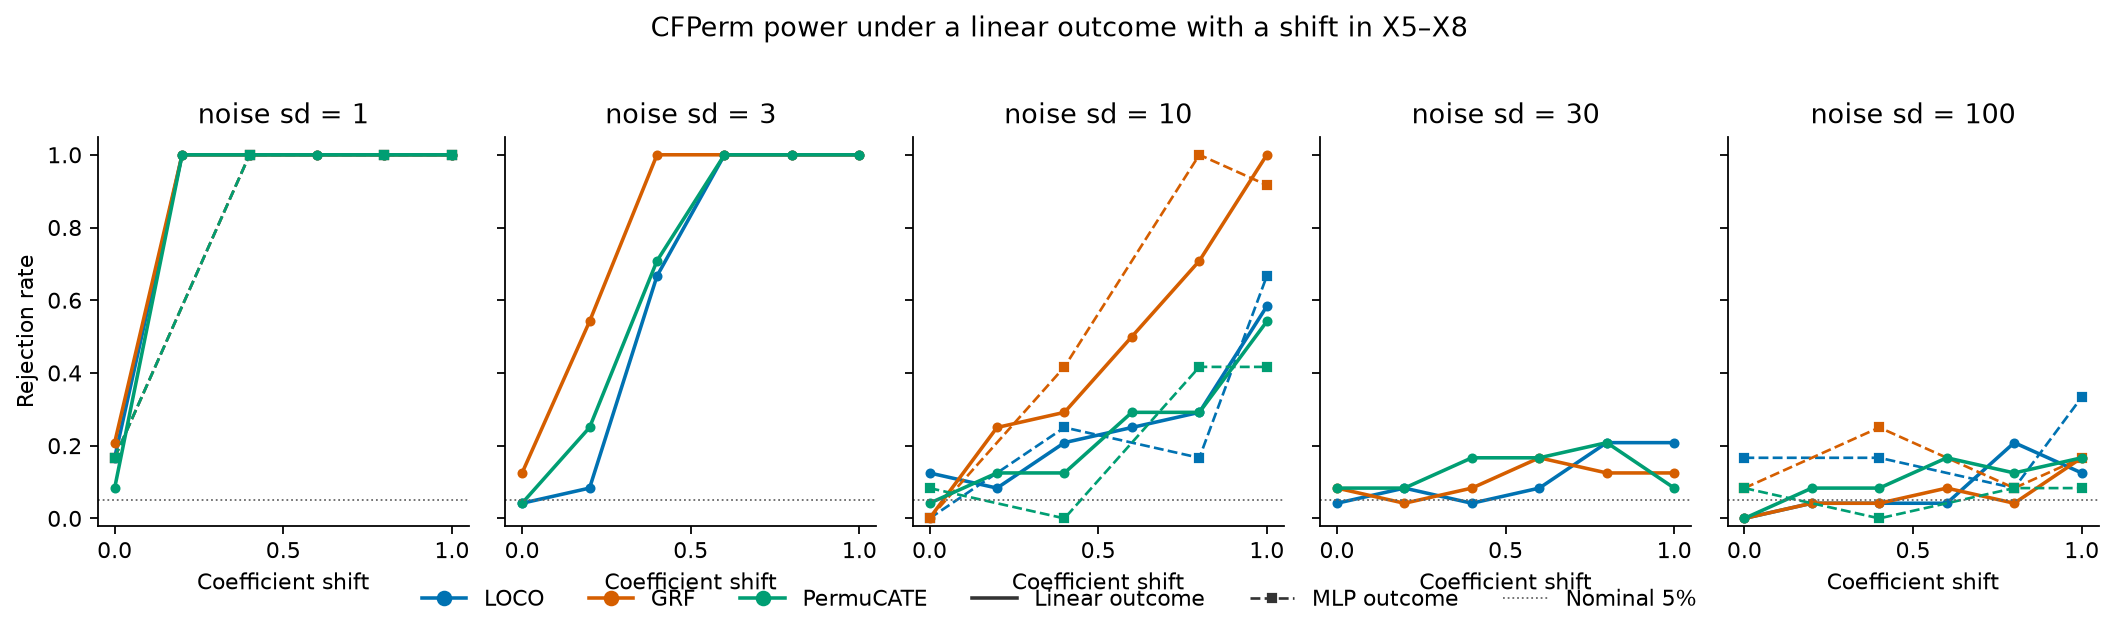
\includegraphics[width=\textwidth]{power_curves.png}
\caption{Rejection rate against the coefficient shift.
Solid lines are the linear outcome.
Dashed lines are the network, on the noise levels where it was run.
The propensity in the figure is logistic.
The dotted line is the nominal \(5\%\) level.}
\label{fig:lm-power}
\end{figure}

At \(\sigma=1\), LOCO, GRF, and PermuCATE agree.
A zero shift rejects in \(0.17\), \(0.21\), and \(0.08\) of replicates.
A shift of \(0.2\) rejects in every replicate, and every rejection names a
shifted coordinate.
The same agreement holds out to a unit shift.
At \(\sigma=3\) the three curves still meet, at a shift of \(0.6\): each
rejects in every replicate and names the shifted coordinates.
GRF is ahead on the smaller shifts (\(0.54\) at \(\delta=0.2\), \(1.00\) at
\(\delta=0.4\)).
At \(\sigma=10\) the order is the same one and it is monotone in the shift.
A unit shift has power \(1.00\) for GRF, \(0.58\) for LOCO, and \(0.54\) for
PermuCATE, with signal rates \(1.00\), \(0.54\), and \(0.46\).
At \(\sigma=30\) and \(\sigma=100\) the three notions sit together between
\(0\) and \(0.21\), which is the same range as their null cells.
The curves in Figure~\ref{fig:lm-power} do not cross once the noise is large.

\begin{table}[p]
\centering
\small
\caption{Linear outcome, logistic propensity.
Each cell is the rejection rate, with the shifted-feature hit rate in
parentheses.
Rows are residual standard deviation and coefficient shift.
\(B=24\), \(49\) permutations.}
\label{tab:lm-logistic}
\begin{tabular}{llccc}
\toprule
\(\sigma\) & \(\delta\) & LOCO & GRF & PermuCATE \\
\midrule
1 & 0.0 & 0.17 (0.00) & 0.21 (0.04) & 0.08 (0.00) \\
1 & 0.2 & 1.00 (1.00) & 1.00 (1.00) & 1.00 (1.00) \\
1 & 0.4 & 1.00 (1.00) & 1.00 (1.00) & 1.00 (1.00) \\
1 & 0.6 & 1.00 (1.00) & 1.00 (1.00) & 1.00 (1.00) \\
1 & 0.8 & 1.00 (1.00) & 1.00 (1.00) & 1.00 (1.00) \\
1 & 1.0 & 1.00 (1.00) & 1.00 (1.00) & 1.00 (1.00) \\
\midrule
3 & 0.0 & 0.04 (0.00) & 0.12 (0.00) & 0.04 (0.04) \\
3 & 0.2 & 0.08 (0.08) & 0.54 (0.46) & 0.25 (0.25) \\
3 & 0.4 & 0.67 (0.67) & 1.00 (1.00) & 0.71 (0.71) \\
3 & 0.6 & 1.00 (1.00) & 1.00 (1.00) & 1.00 (1.00) \\
3 & 0.8 & 1.00 (1.00) & 1.00 (1.00) & 1.00 (1.00) \\
3 & 1.0 & 1.00 (1.00) & 1.00 (1.00) & 1.00 (1.00) \\
\midrule
10 & 0.0 & 0.12 (0.04) & 0.00 (0.00) & 0.04 (0.00) \\
10 & 0.2 & 0.08 (0.00) & 0.25 (0.04) & 0.12 (0.08) \\
10 & 0.4 & 0.21 (0.04) & 0.29 (0.25) & 0.12 (0.08) \\
10 & 0.6 & 0.25 (0.12) & 0.50 (0.50) & 0.29 (0.25) \\
10 & 0.8 & 0.29 (0.17) & 0.71 (0.71) & 0.29 (0.21) \\
10 & 1.0 & 0.58 (0.54) & 1.00 (1.00) & 0.54 (0.46) \\
\midrule
30 & 0.0 & 0.04 (0.04) & 0.08 (0.00) & 0.08 (0.04) \\
30 & 0.2 & 0.08 (0.00) & 0.04 (0.04) & 0.08 (0.00) \\
30 & 0.4 & 0.04 (0.00) & 0.08 (0.04) & 0.17 (0.00) \\
30 & 0.6 & 0.08 (0.00) & 0.17 (0.04) & 0.17 (0.04) \\
30 & 0.8 & 0.21 (0.08) & 0.12 (0.04) & 0.21 (0.08) \\
30 & 1.0 & 0.21 (0.08) & 0.12 (0.04) & 0.08 (0.04) \\
\midrule
100 & 0.0 & 0.00 (0.00) & 0.00 (0.00) & 0.00 (0.00) \\
100 & 0.2 & 0.04 (0.04) & 0.04 (0.04) & 0.08 (0.08) \\
100 & 0.4 & 0.04 (0.00) & 0.04 (0.00) & 0.08 (0.00) \\
100 & 0.6 & 0.04 (0.00) & 0.08 (0.00) & 0.17 (0.00) \\
100 & 0.8 & 0.21 (0.08) & 0.04 (0.00) & 0.12 (0.00) \\
100 & 1.0 & 0.12 (0.04) & 0.17 (0.04) & 0.17 (0.04) \\
\bottomrule
\end{tabular}
\end{table}

Replacing the linear outcome by the network does not move the cells where
the linear fit already has power \(1\).
At \(\sigma=1\) and \(\delta\in\{0.4,0.8,1\}\) both outcome models reject in
every replicate, for all three notions.
At \(\sigma=10\) and a unit shift the pairs are \(0.58/0.67\) (LOCO),
\(1.00/0.92\) (GRF), and \(0.54/0.42\) (PermuCATE), linear over network.
At \(\sigma=100\) both sit near the null.
The largest gap on that slice is LOCO at a unit shift, \(0.12\) against
\(0.33\), on \(12\) network replicates.
Table~\ref{tab:lm-mlp} is the whole overlapping grid.

\begin{table}[t]
\centering
\small
\caption{Linear outcome over network outcome, logistic propensity.
Each cell is the linear rejection rate over the network rejection rate,
on the shift values the network was run.
The linear rate uses \(B=24\).
The network rate uses \(B=12\).}
\label{tab:lm-mlp}
\begin{tabular}{llccc}
\toprule
\(\sigma\) & \(\delta\) & LOCO & GRF & PermuCATE \\
\midrule
1 & 0.0 & 0.17/0.17 & 0.21/0.17 & 0.08/0.17 \\
1 & 0.4 & 1.00/1.00 & 1.00/1.00 & 1.00/1.00 \\
1 & 0.8 & 1.00/1.00 & 1.00/1.00 & 1.00/1.00 \\
1 & 1.0 & 1.00/1.00 & 1.00/1.00 & 1.00/1.00 \\
\midrule
10 & 0.0 & 0.12/0.00 & 0.00/0.00 & 0.04/0.08 \\
10 & 0.4 & 0.21/0.25 & 0.29/0.42 & 0.12/0.00 \\
10 & 0.8 & 0.29/0.17 & 0.71/1.00 & 0.29/0.42 \\
10 & 1.0 & 0.58/0.67 & 1.00/0.92 & 0.54/0.42 \\
\midrule
100 & 0.0 & 0.00/0.17 & 0.00/0.08 & 0.00/0.08 \\
100 & 0.4 & 0.04/0.17 & 0.04/0.25 & 0.08/0.00 \\
100 & 0.8 & 0.21/0.08 & 0.04/0.08 & 0.12/0.08 \\
100 & 1.0 & 0.12/0.33 & 0.17/0.17 & 0.17/0.08 \\
\bottomrule
\end{tabular}
\end{table}

The propensity model is the other nuisance.
The two batches have the same covariate law and a balanced label, so the
propensity is a constant near one half.
Table~\ref{tab:lm-ridge} compares logistic with binomial ridge on the
corner cells, linear over ridge.
At \(\sigma=1\) and a unit shift every notion rejects in every replicate
under both propensities.
At \(\sigma=10\) and a unit shift, LOCO is \(0.58/0.56\) and GRF is
\(1.00/1.00\).
PermuCATE is \(0.54/0.25\).
That is the one cell in the corner grid where the propensity changes the
rate by more than sampling noise: the ridge cell has \(16\) replicates.
Null cells stay inside \(0.00\)--\(0.21\) for every propensity, notion, and
noise level in the two tables.

\begin{table}[t]
\centering
\small
\caption{Logistic propensity over binomial ridge, linear outcome.
Corner cells of the shift grid.
The logistic rate uses \(B=24\).
The ridge rate uses \(B=16\).}
\label{tab:lm-ridge}
\begin{tabular}{llccc}
\toprule
\(\sigma\) & \(\delta\) & LOCO & GRF & PermuCATE \\
\midrule
1 & 0.0 & 0.17/0.12 & 0.21/0.12 & 0.08/0.06 \\
1 & 1.0 & 1.00/1.00 & 1.00/1.00 & 1.00/1.00 \\
10 & 0.0 & 0.12/0.06 & 0.00/0.12 & 0.04/0.12 \\
10 & 1.0 & 0.58/0.56 & 1.00/1.00 & 0.54/0.25 \\
\bottomrule
\end{tabular}
\end{table}

The linear outcome is enough for this shift.
Where the signal is large relative to the residual, LOCO, GRF, and
PermuCATE give the same rejection, and swapping in the network does not
raise it.
Where the residual standard deviation reaches \(30\), the three notions
lose the shift together.
